\chapter{Dimensionering af stålprofiler}

Figur \ref{fig:hej} viser de nye byggefelter inden for henholdsvis delområde A og delområde B til Strøybergs Palæ (\citep{lokalplan}, s. 16). Denne rapport fokuserer på byggefeltet inden for delområde B, hvor ny bebyggelse, ifølge lokalplan 1-1-107, må opføres i 3 etager samt en tagetage og med en kælder maksimalt 2 m over terræn. Ved opførsel af ny bebyggelse i delområde B, skal to nuværende mindre bygninger fjernes. 

\begin{figure}[htbp]
	\centering
	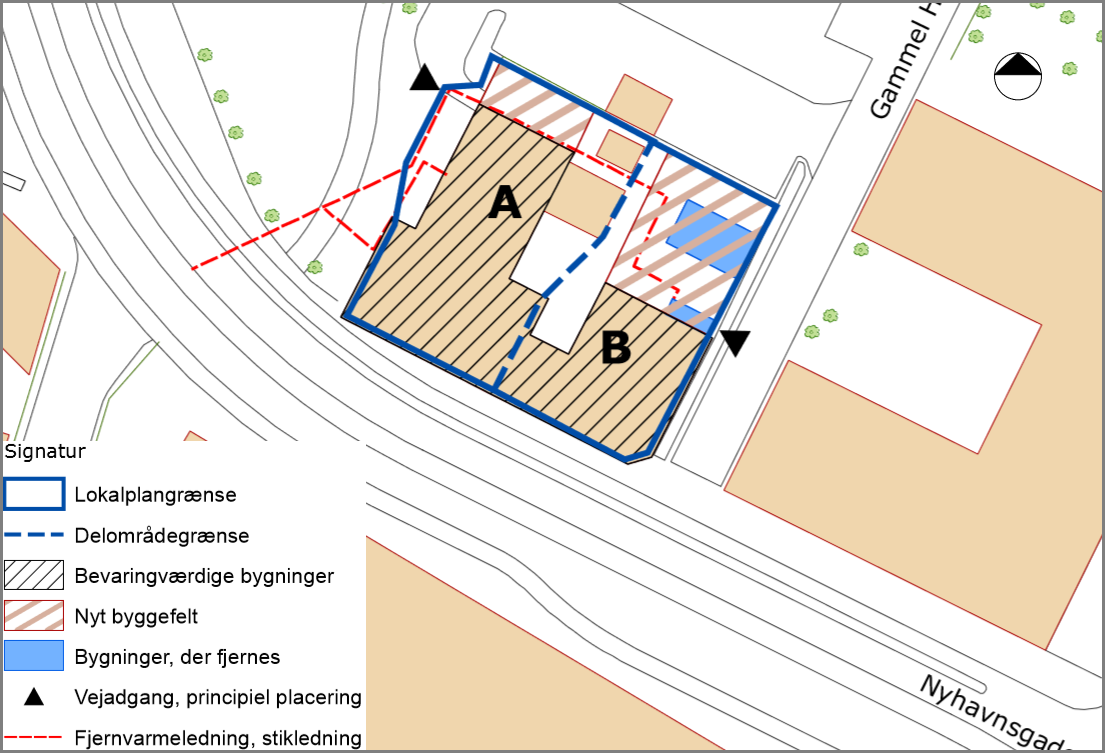
\includegraphics[width=0.8\textwidth]{billeder/signatur.png}
	\caption{Lokalplan 1-1-107, delområde A og B \citep[ bilag 2, s. 35]{lokalplan}}
	\label{fig:hej}
\end{figure}

Med udgangspunkt i lokalplan 1-1-107 har bygningen fået de størrelser og dimensioner, som ses på Figur \ref{fig:farvel}, som videre beregninger tager udgangspunkt i.
\newline \indent{     }  Tilbygningen sættes til at være $12,\!5$ m lang og 12 m bred i henhold til den eksisterende bygningsbredde. Kælderen har en højde på i alt $3,\!25$ m, hvor $1,\!25$ m ligger over terræn. Stueetagen, 1. sal og 2. sal har hver især en højde på $4,\!9$ m og tagetagen har en højde på 3 meter med en hældning på $26,\!57^{\circ}$. I alt er tilbygningen 19 m høj over terræn.

\begin{figure}[H]
	\centering
	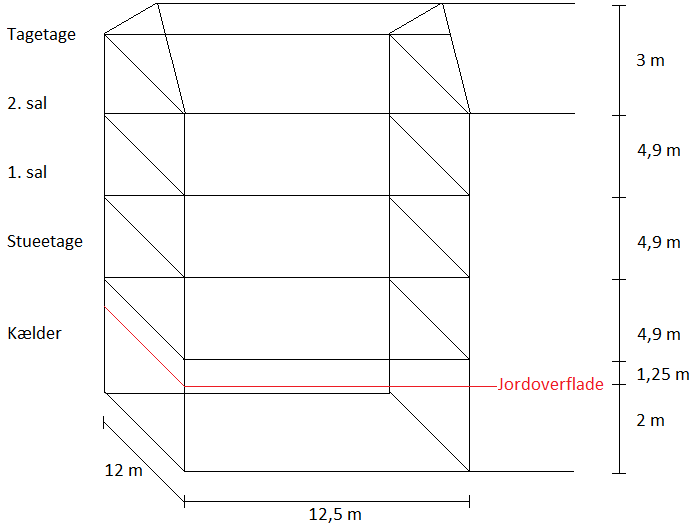
\includegraphics[width=0.8\textwidth]{billeder/tilbygning2.png}
	\caption{Tilbygningens dimensioner}
	\label{fig:farvel}
\end{figure}

For at kunne beregne de laster som påvirker tilbygningen, er der opstillet et statisk system som ses på Figur \ref{fig:system}. Systemet er opstillet som en bjælkekonstruktion. Som det ses på Figur \ref{fig:farvel} er der tre stålrammer; en i midten og en i hver af gavlene. I videre beregninger foretages der beregninger for rammen i midten.

\begin{figure}[H]
	\centering
	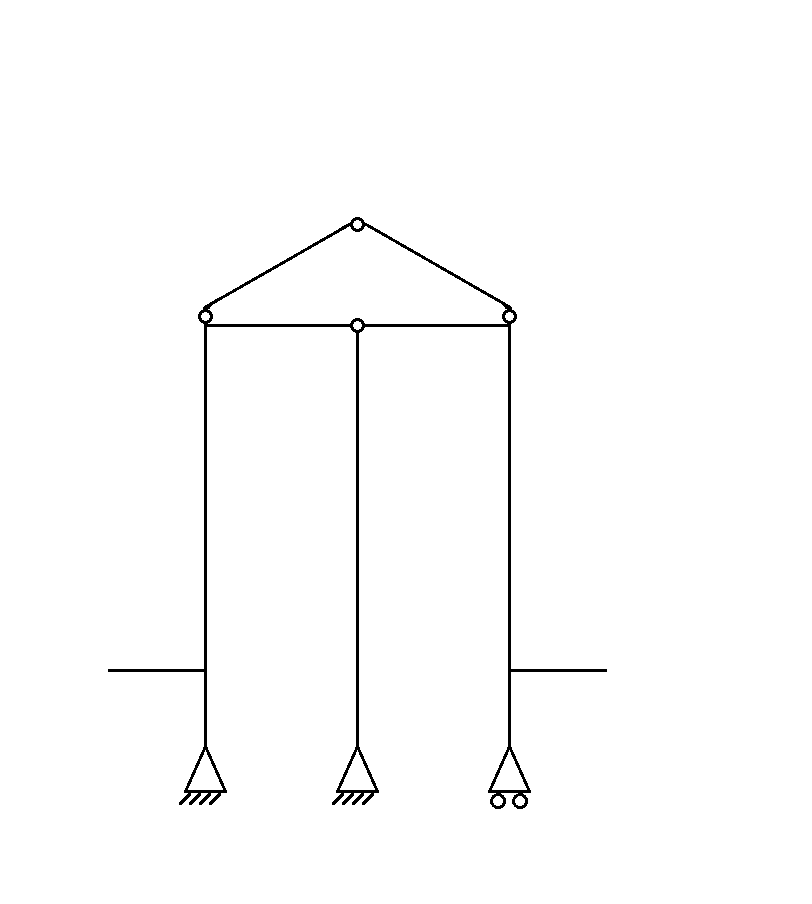
\includegraphics[width=0.4\textwidth]{billeder/del1statiskesystem.png}
	\caption{Statisk system}
	\label{fig:system}
\end{figure}

Etagedækkene vil virke som en belastning, og ses ikke som en del af konstruktionen. Dette er muligt, da der opsættes en samling mellem etagedækkene og stålkonstruktion, som ses på Figur \ref{fig:etage}.

\begin{figure}[H]
	\centering
	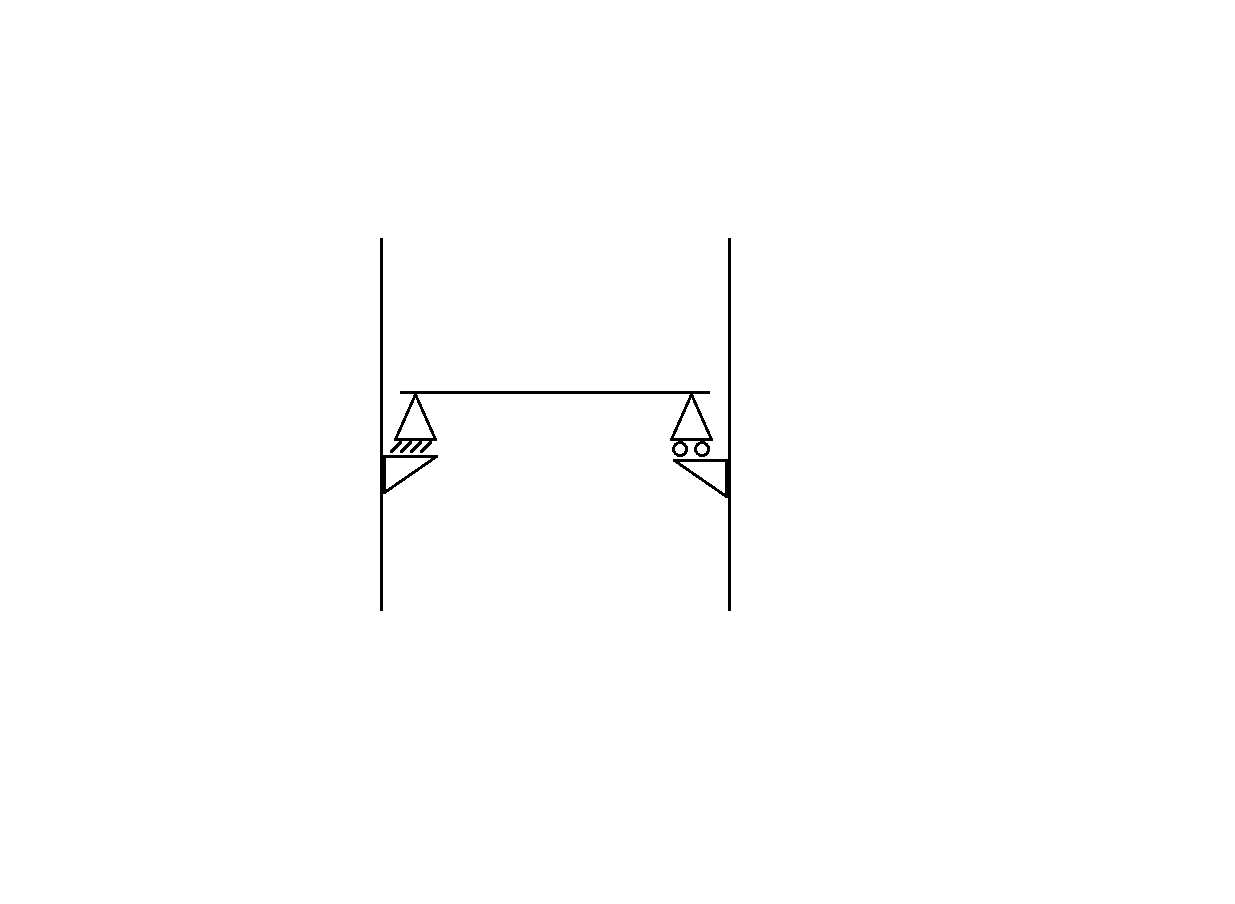
\includegraphics[width=0.3\textwidth]{billeder/etageovergang.png}
	\caption{Etageovergang på tilbygningen}
	\label{fig:etage}
\end{figure}

Ståltypen for det statiske system sættes til at være ståltype S235 med I-profil nr. 450 \citep{stabi}. Mål for profilet ses på Figur \ref{fig:iprofil}. 

\section{Laster}
Tilbygningen til Strøybergs Palæ vil blive udsat for en række laster, både permanente- og variable laster. Disse vil blive beregnet i dette afsnit, så der kan opstilles lastkombinationer samt beregnes brudgrænse- og anvendelsesgrænsetilstande.

\subsection{Permanente laster}
De permanente laster, der beregnes er egenlast og jordlast.

\subsubsection{Egenlast}
For at bestemme den egenlast, der virker på det statiske system, beregnes først en samlet egenlast for taget, dernæst bestemmes egenlasten for gulve og vægge, hvorudfra den samlede egenlast for etagerne kan bestemmes. Til sidst bestemmes egenlasten for stålsystemet ekslusivt tag. Den egenlast, der virker under taget opdeles altså i egenlast fra stålsystem og egenlast fra etagedæk, idet egenlasten fra etagedækkene giver anledning til moment, grundet samlingen mellem etagedækkene og stålkonstruktionen, som ses på Figur \ref{fig:etage}. 
\newline \indent{     }  Lasterne deles ud på de tre rammer, hvor den midterste optager halvdelen af lasterne. De bestemte laster laves til sidst om til linjelaster, som sættes på bjælkesystemet.  

\textbf{Last fra tag}
\newline
Det antages, at taget er et mellemtungt sadeltag med teglsten, som har egenvægten \SI{600}{$\frac{\text{N}}{\text{m}^2}$} \citep{tag}.
\newline
\newline
Tagets areal bestemmes ud fra Figur \ref{fig:tagetage}:
\begin{equation}
	A_{tag} = \SI{6,71}{m} \cdot \SI{12,50}{m} \cdot 2 = \SI{167,71}{m^2}
\end{equation}

Arealet multipliceres med egenvægten for mellemtungt tag, for at finde lasten for hele taget på tilbygningen:
\begin{equation}
	p_{tag} = \SI{167,71}{m^2}\cdot \SI{600}{$\frac{\text{N}}{\text{m}^2}$} = \SI{100,62}{kN}
\end{equation}

Denne last vil blive fordelt ud på de tre rammer (se Figur \ref{fig:farvel}), hvor den midterste ramme vil optage halvdelen af lasten, som herefter omregnes til en linjelast:
\begin{equation}
	\frac{\frac{100,62\text{kN}}{2}}{6,\!71\text{m} \cdot2} = 3,\!75
	\frac{\text{kN}}{\text{m}}
\end{equation}

Denne værdi skal lægges sammen med egenlasten for stålsystemet i tagkonstuktionen, for at bestemme den samlede egenlast for taget.
\newline \indent{     }  Egenlasten for stålet regnes ud fra densiteten for det anvendte profil nr. 450. Her er densiteten \SI{115}{$\frac{\text{kg}}{\text{m}}$} \citep{stabi}. Denne multipliceres med tyngdeaccelerationen, for at få en linjelast:
\begin{equation}
	\SI{115}{$\frac{\text{kg}}{\text{m}}$} \cdot \SI{9,82}{$\frac{\text{m}}{\text{s}^2}$} = \SI{1,13}{$\frac{\text{kN}}{\text{m}}$}
\end{equation}

Denne linjelast kan nu adderes til tagets egenlast, og den samlede egenlast for taget er bestemt til \SI{4,89}{$\frac{\text{kN}}{\text{m}}$}.

\begin{figure}[H]
	\centering
	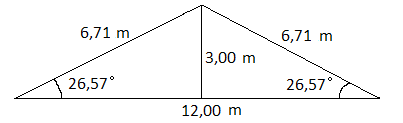
\includegraphics[width=0.5\textwidth]{billeder/Tagmedvinkel.png}
	\caption{Dimensioner for tagetagen}
	\label{fig:tagetage}
\end{figure}

\textbf{Last fra vægge}
\newline
Egenlasten for etagerne udregnes nu, ved først at regne egenlasten for væggene. Tilbygningens to facader antages at være ens, og hver især bestå af 11 vinduer og én dør \citep{gammellokalplan}, hvilket illustreres på Figur \ref{fig:facade}.

\begin{figure}[H]
	\centering
	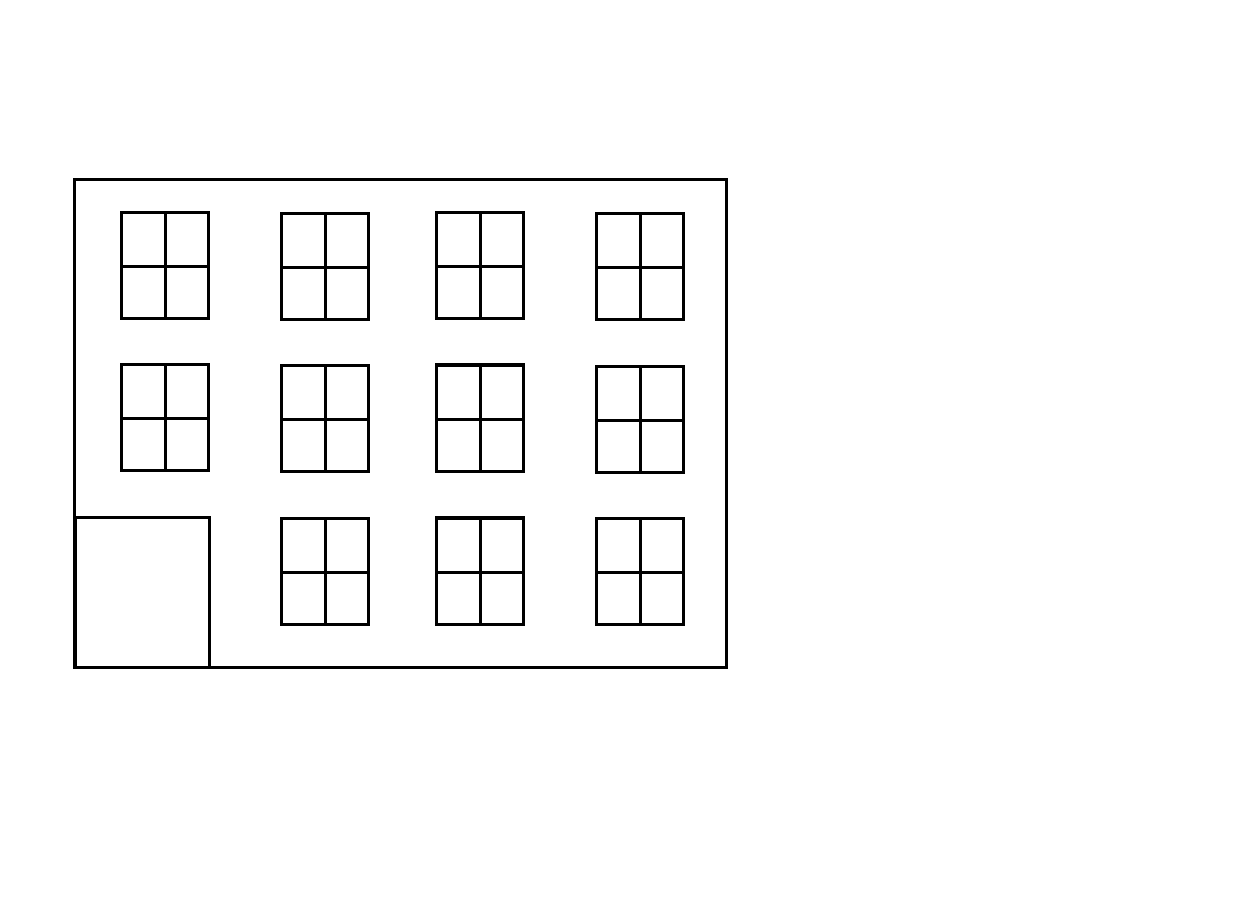
\includegraphics[width=0.6\textwidth]{billeder/facadenord.png}
	\caption{Facaden på øst- og vestsiden}
	\label{fig:facade}
\end{figure}

Til beregning af væggens egenlast skal der påregnes en indervæg og et isoleringslag. Ydervæggen bærer sig selv, og er derfor ikke er en del af det statiske system, og skal derfor ikke medregnes. Indervæggen bestemmes at være mursten, og isoleringen bestemmes at være rockwool. Tykkelsen og densiteten for mursten og rockwool kan ses på Figur \ref{fig:vaeg}.

\begin{figure}[H]
	\centering
	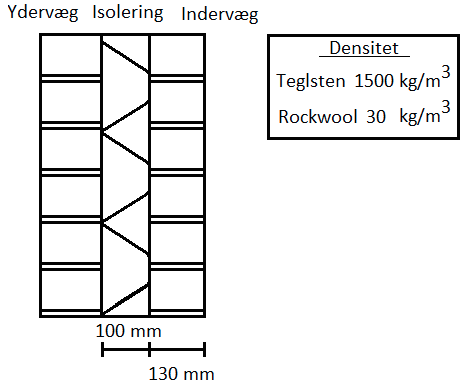
\includegraphics[width=0.5\textwidth]{billeder/mur.png}
	\caption{Opbygning af væg}
	\label{fig:vaeg}
\end{figure}

Der medregnes kun egenlast for én gavl, idet den anden gavl ligger op ad den nuværende bygning, og den belaster dermed ikke det statiske system. 
\newline \indent{     }  De ni vinduer på gavlen har identiske mål med dem på facaden, som kan ses på Figur \ref{fig:gavl}. Indervæg og isolering for gavlen er ligeledes identisk med facadens.
\newline \indent{     }  Når arealet af facaderne beregnes trækkes arealet af vinduerne samt døren fra, da disse antages at belaste ydermuren.

\begin{figure}[H]
	\centering
	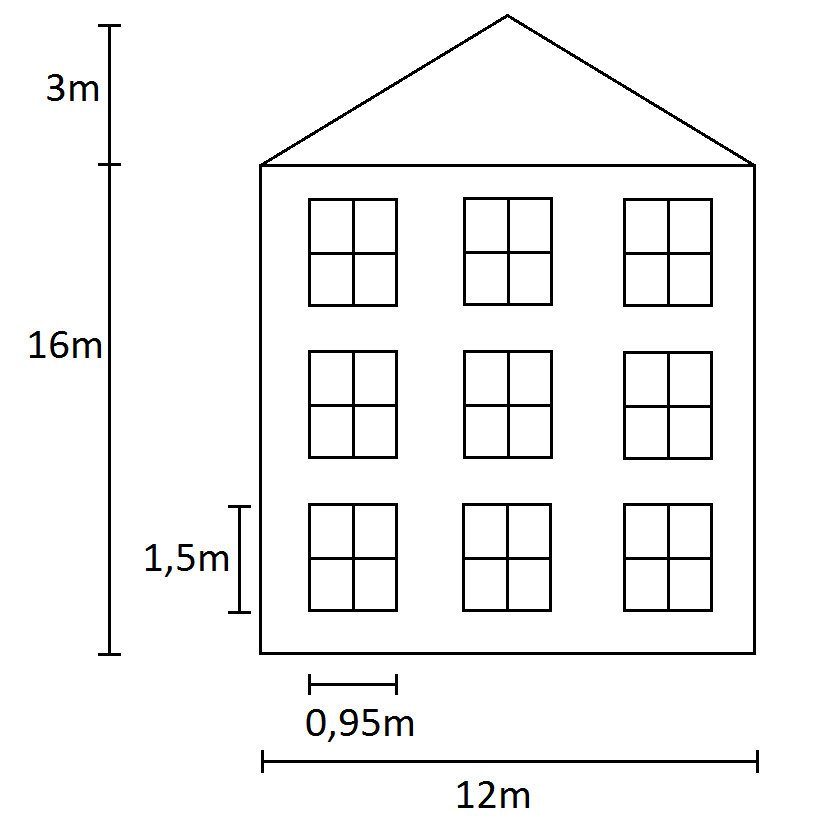
\includegraphics[width=0.4\textwidth]{billeder/facadevestellerost.png}
	\caption{Mål og dimensioner for gavl og tilbygningen}
	\label{fig:gavl}
\end{figure}

Arealerne og lasten for facaderne og gavlen kan ses i Tabel \ref{tab:arealoglast}, hvor lasten bestemmes ud fra formlen:
\begin{equation}
	p = g A \sum dt
\end{equation}

\begin{itemize}
	\item[-] $g$: Tyngdeacceleration på \SI{9,82}{$\frac{\text{m}}{\text{s}^2}$}
	\item[-] $A$: Areal
	\item[-] $d$: Densitet af materiale
	\item[-] $t$: Tykkelse af materiale
\end{itemize}

\begin{table} [H]
	\begin{center}
		\begin{tabular}{c c c }
			\hline
			Retning & Areal   & Last    \\
			& \textit{A} [$\text{m}^2$] & \textit{p} [kN] \\ \hline
			Facade, vest & 181,18 & 352,27 \\
			Facade, øst  & 181,18 & 352,27 \\
			Gavl, nord   & 197,18 & 383,38 \\
		\end{tabular}
		\caption{Areal og last for væg}
		\label{tab:arealoglast}
	\end{center}
\end{table}

\textbf{Last fra gulv}
\newline
Det antages, at bygningens etager kun består af gulv, dvs. ingen skillevægge, trapper m.m. Derfor er det samlede areal af gulvet pr. etage: 
\begin{equation}
	A_{etage} = \SI{12,50}{m} \cdot \SI{12,00}{m} = \SI{150,00}{$\text{m}^2$}
\end{equation}

Fire ud af tilbygningens fem etager består af bærende gulve. Kælderetagen ligger på fundamentet, og bliver dermed ikke båret af rammen. Derfor medregnes kælderetagens gulv ikke i egenlasten. 
\newline \indent{     }  Opbygningen af det bærende gulv er illustreret på Figur \ref{fig:gulv}. Det bærende gulv består af et armeret betondæk nederst, der oftest er mellem 80 mm og 200 mm tyk. Det bestemmes, at den er 120 mm tyk, hvorpå der ligger strøer. Strøernes opgave er at løfte gulvet, således der er plads til isoleringslaget \citep{Gulvopbygning}. Densiteten og tykkelsen af gulvlagene kan ses i Tabel \ref{tab:densi}.

\begin{figure}[H]
	\centering
	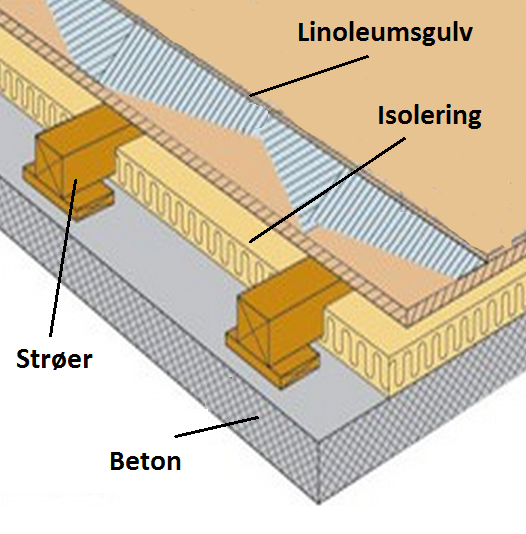
\includegraphics[width=0.6\textwidth]{billeder/gulv.png}
	\caption{Opbygning af bærende gulv \citep{gulv} \citep{granse}}
	\label{fig:gulv}
\end{figure}

Der er behov for strøer, som hver er $6,\!25$ m lange. Disse anlægges langs med tilbygningen, og antallet af strøer bestemmes ved at dividere med 400 mm, da der anbefales at være 400 mm imellem hver strø \citep{Gulvopbygning}. 
\begin{equation}
	\frac{2\cdot 6,\!25 \text{m}}{0,\!40 \text{m}} = \SI{31,25}{\text{strøer}}
\end{equation} 

Dette afrundes til 32 strøer.


Nu bestemmes egenlasten for strøerne ved at multiplicere 32 strøer med deres rumfang samt densitet, for tørrumvægt af træ 510 [$\frac{\text{kg}}{\text{m}^3}$] \citep{torrumvagt}, tyngdeaccelerationen og fire etager:
\begin{equation}
	p_{\textup{strøer}} = \SI{7,84}{m^3} \cdot 510 [\frac{\text{kg}}{\text{m}^3}] \cdot 9,\!82 \frac{\text{m}}{\text{s}^2} \cdot 4 = \SI{157,06}{kN}
\end{equation}

Udregningen af volumen og egenlast for beton, rockwool og linoleum sker på samme måde som for strøerne, dog skal strøernes volumen trækkes fra ved beregning af værdierne for rockwool. Resultaterne kan ses i Tabel \ref{tab:densi}.

\begin{table} [H]
	\begin{center}
		\begin{tabular}{c c c c}
			\hline
			Materiale & Densitet & Volumen & Last \\
			& \textit{d} [$\frac{\text{kg}}{\text{m}^3}$] & \textit{V} [$\text{m}^3$] & \textit{p} [kN] \\ \hline
			Strøer & - & 7,84 & 157,06	\\
			Beton    & 2400 & 72,00 & 1693,44      \\ 
			Rockwool & 30  & 52,64 & 15,51     \\ 
			Linoleum & 2,9 & 1,50 & 0,04 \\ 
		\end{tabular}
		\caption{Materialer og deres egenskaber for gulv}
		\label{tab:densi}
	\end{center}
\end{table}

\textbf{Samlet egenlast for etagedæk}
\newline
Lasterne fra henholdsvis Tabel \ref{tab:arealoglast} og Tabel \ref{tab:densi} adderes, og der fås en samlet egenlast for tilbygningen på $2953,\!90$ kN. 
\newline \indent{     }  Denne deles med 2, da midterrammen i tilbygningen optager halvdelen af den samlede egenlast, og der fås $1476,\!95$ kN. 
\newline
\newline
Den midterste bjælke i det statiske system optager halvdelen af egenlasten, mens de to yderste bjælker hver optager en fjerdedel:
\begin{equation}
	\frac{1476,\!95 \text{kN}}{4} = \SI{369,24}{kN}
\end{equation}

Punktlasten for egenlasten omregnes nu til en linjelast, ved at dele med højden 18 m:
\begin{equation}
	\frac{369,\!24 \text{kN}}{18 \text{m}} = \SI{20,51}{$\frac{\text{kN}}{\text{m}}$}
\end{equation}

Egenlasten fra etagedækkene, der påvirker bjælkerne, er dermed $20,\!51 \frac{\text{kN}}{\text{m}}$ for de to yderste bjælker og 41,03 $\frac{\text{kN}}{\text{m}}$ for den midterste bjælke. 

\textbf{Egenlast af stålsystemet}
\newline
Der beregnes en egenlast for stålsystemet ekslusivt tag. 
\newline
\newline
For at finde linjelasten af en stålbjælke multipliceres profilets densitet 115,00 $\frac{\text{kg}}{\text{m}}$ med tyngeaccelerationen:
\begin{equation}
	115,\!00 \frac{\text{kg}}{\text{m}} \cdot 9,\!82 \frac{\text{m}}{\text{s}^2} = 1,\!13 \frac{\text{kN}}{\text{m}}
\end{equation}

\textbf{Opsamling}
\newline
De karakteristiske egenlaster fra henholdsvis taget, etagedækkene samt stålsystemet er nu bestemt. Disse placeres nu i det statiske system vist på Figur \ref{fig:m} og \ref{fig:n}.

\begin{figure}[H]\centering
	\begin{minipage}[b]{0.48\textwidth}\centering
		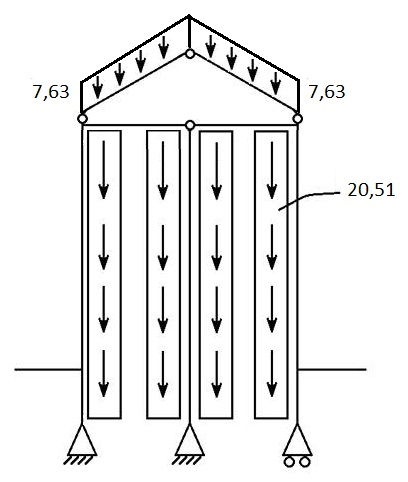
\includegraphics[width=0.80\textwidth]{billeder/egenlastetage.png} %Venstre billede
	\end{minipage}\hfill
	\begin{minipage}[b]{0.48\textwidth}\centering
		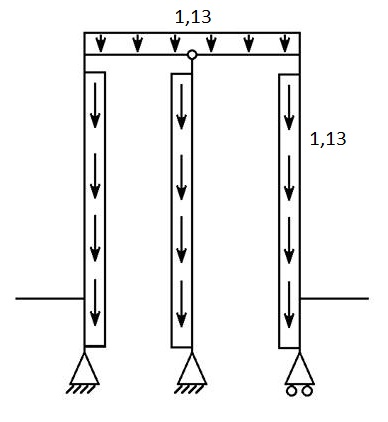
\includegraphics[width=0.8\textwidth]{billeder/egenlaststaal.png} %Højre billede
	\end{minipage}\\ %Captions and labels
	\begin{minipage}[t]{0.48\textwidth}
		\caption{Egenlast fra etagedæk angivet i [$\frac{\text{kN}}{\text{m}}$]} %Venstre caption og label
		\label{fig:m}
	\end{minipage}\hfill
	\begin{minipage}[t]{0.48\textwidth}
		\caption{Egenlast fra stålsystemet angivet i [$\frac{\text{kN}}{\text{m}}$]} %Højre caption og label
		\label{fig:n}
	\end{minipage}
\end{figure}

\subsubsection{Jordlast}
Idet tilbygningen har en kælder, der går 2 m under jorden, bliver den påvirket med en jordlast. Jordlasten virker på konstruktionen fra jordoverfladen og nedefter, og virker liniært afhængigt af dybden.
\newline
\newline
Jordlasten beregnes gennem formlen:
\begin{equation}
	\sigma_x = k_0 \sigma_z
\end{equation}

\begin{itemize}
	\item[-] $k_0$: Hviletrykskoefficienten, som er givet ved $k_0=1-\sin(\varphi)$, hvor $\varphi$ er friktionsvinklen. Friktionsvinklen er bestemt igennem fire laboratorieforsøg, som ses under afsnit 10.2.5. 
	\item[-] $\sigma_z$: Den lodrette fladelast i dybden $z$ givet ved $\sigma_z = z\gamma$, hvor $z$ er dybden og $\gamma$ er rumvægten $[\frac{\text{kN}}{\text{m}^3}]$
\end{itemize}

Hviletrykskoefficenten, $k_0$ bestemmes:
\begin{equation}
	k_0 = 1 - \sin(32,\!33) = 0,\!47
\end{equation}

Rumvægten slås op til 20 $\frac{\text{kN}}{\text{m}^3}$ \citep[ s. 386]{stabi} og den lodrette hviletryksspænding, $\sigma_z$, bestemmes:
\begin{equation}
\sigma_z = z\cdot 20 \frac{\text{kN}}{\text{m}^3}
\end{equation}

Nu er hviletrykskoefficienten og fladlasten bestemt, og det betyder, at jordlasten $\sigma_x$, i dybderne $z$ for 0 m og 2 m bestemmes:
\begin{equation}
\sigma_x = 0,\!47\cdot \SI{0}{m}\cdot 20 \frac{\text{kN}}{\text{m}^3} = 0 \frac{\text{kN}}{\text{m}^2}
\end{equation}

\begin{equation}
	\sigma_x = 0,\!47\cdot \SI{2}{m}\cdot 20 \frac{\text{kN}}{\text{m}^3} = 18,\!61 \frac{\text{kN}}{\text{m}^2}
\end{equation}

I og med jordlasten ved 0 m er 0 $\frac{\text{kN}}{\text{m}^2}$, vil den også optræde som en linjelast med værdien 0 $\frac{\text{kN}}{\text{m}^2}$. Dermed beregnes linjelasten for dybden 2 m, ved at multiplicere med længden, som den virker over, hvilken er 6,25 m:
\begin{equation}
	q_{x,linje} = 18,\!61 \frac{\text{kN}}{\text{m}^2}\cdot \SI{6,25}{m} = 116,\!32 \frac{\text{kN}}{\text{m}}
\end{equation}

Jordlasten virker derfor som en lineær funktion, og der opstilles nu et generelt udtryk for funktionen $j(z)$: 
\begin{equation}
	j(z) = a z + b
\end{equation}

\begin{itemize}
	\item[-] $a$: Hældning, som er givet ved $\frac{116,32 \frac{\text{kN}}{\text{m}}}{2 \text{m}} = 58,\!16 \frac{\text{kN}}{\text{m}^2}$
	\item[-] $z$: Koordinatet til jordlasten
	\item[-] $b$: Lasten i $z = 0$ m
\end{itemize}

Linjelasten for jordlasten er derfor givet ved: 
\begin{equation}
	j(z) = 58,\!16 \frac{\text{kN}}{\text{m}^2} \cdot z
\end{equation}

Jordlasten, der virker på det statiske system, er illustreret på Figur \ref{fig:jordlast}.

\begin{figure}[H]
	\centering
	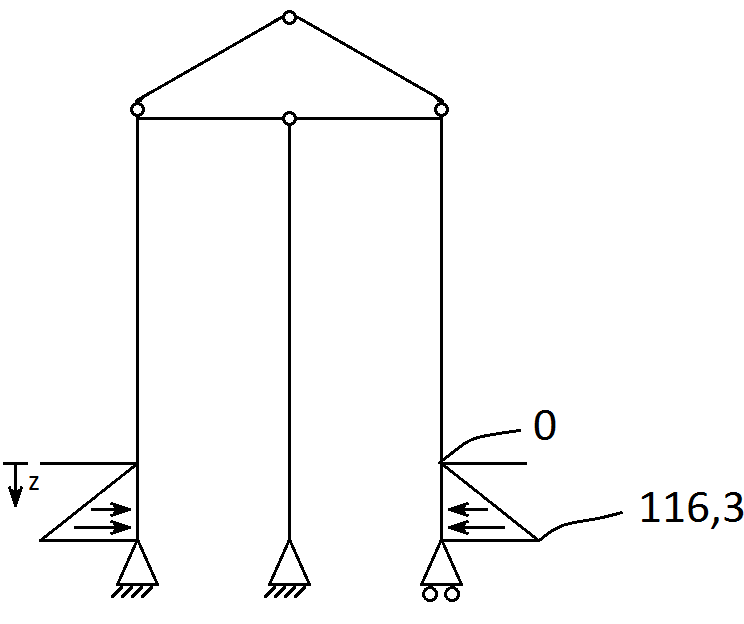
\includegraphics[width=0.5\textwidth]{billeder/jordlast.png}
	\caption{Jordlast på det statiske system angivet i [$\frac{\text{kN}}{\text{m}}$]}
	\label{fig:jordlast}
\end{figure}

\subsection{Variable laster}
Af variable laster optræder snelast, vindlast og nyttelast på bygningen. Disse udregnes efter Eurocode 1991.

\subsubsection{Snelast}
Til at beregne den karakteristiske snelast anvendes følgende formel:
\begin{equation}
	s=\mu_iC_eC_ts_k
\end{equation}
\begin{itemize}
	\item[-] $\mu_i$: Formfaktoren for snelasten, som sættes til 0,8 \citep[ tabel 5.2 kapitel 5.3]{EU91}
	\item[-] $C_e$: Eksponeringsfaktoren
	\item[-] $C_t$: Termisk faktor, som sættes til $1,\!0$ \citep[ kapitel 5.2]{EU91}
	\item[-] $s_k$: Karakteristisk terrænværdi, som sættes til 1 $\frac{\text{kN}}{\text{m}^2}$ \citep[ kapitel 4.1]{EU91}
\end{itemize}

Eksponeringsfaktoren, $C_e$, bestemmes ved:
\begin{equation}
	C_e=C_{top}C_s
\end{equation}
\begin{itemize}
	\item[-] $C_{top}$: Topografifaktor, som sættes til $1,\!0$ \citep[ tabel 5.1 kapitel 5.2]{EU91}
	\item[-] $C_s$: Størrelsesfaktor, som sættes til $1,\!0$ \citep[ kapitel 5.2]{EU91}
\end{itemize}

Eksponeringsfaktoren er altså:
\begin{equation}
	C_e = 1,\!0 \cdot 1,\!0 = 1,\!0
\end{equation}

Strøybergs Palæ har et sadeltag, og dermed skal der tages højde for fire lasttilfælde, som ses på Figur \ref{fig:sne}. Derudover multipliceres snetilfældets værdi med 6,25 m, for at omregne til linjelast.

\begin{figure}[htbp]
	\centering
	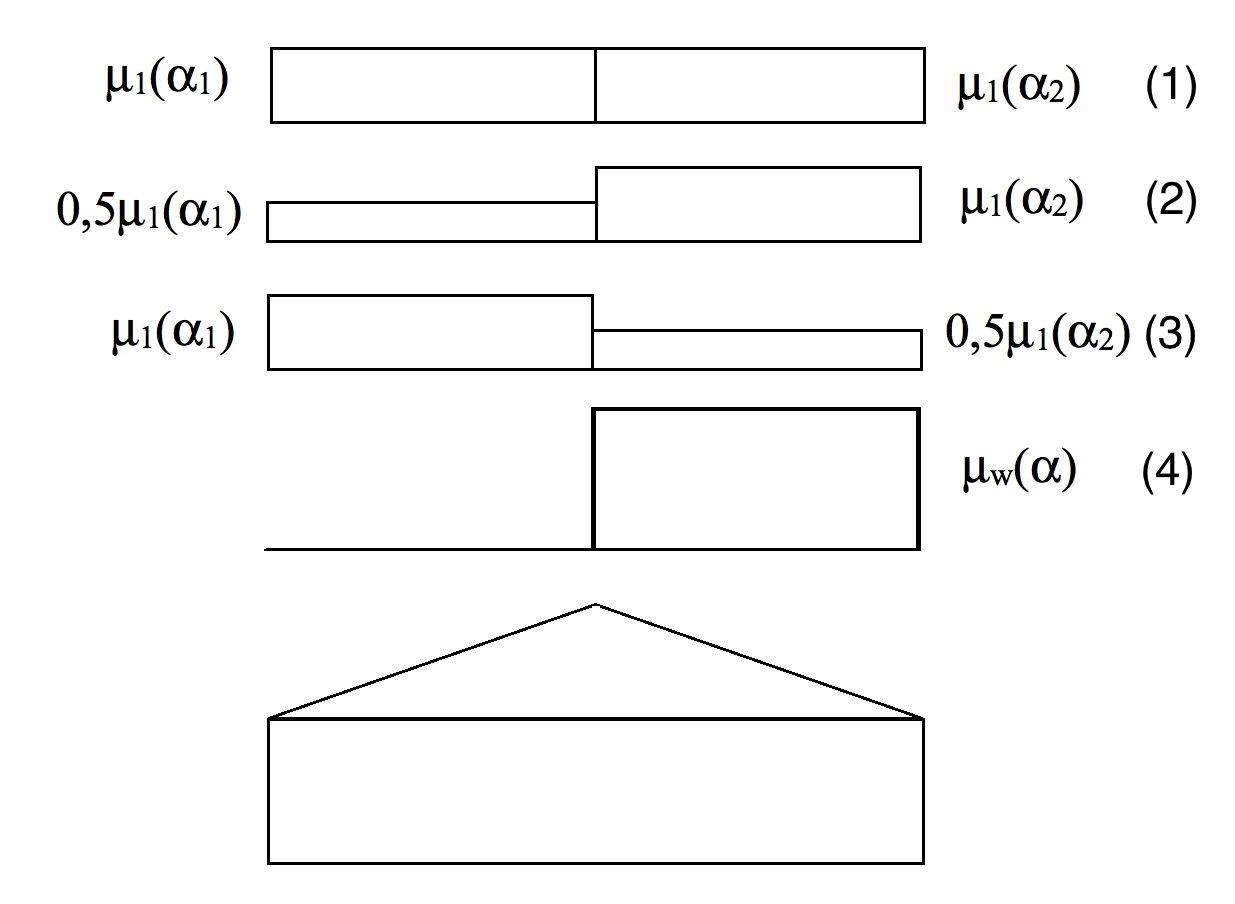
\includegraphics[width=0.6\textwidth]{billeder/snelasttilfaelde.png}
	\caption{Fordeling af sne i de fire tilfælde \citep[ kapitel 5.3.3]{EU91}}
	\label{fig:sne}
\end{figure}

\underline{Snetilfælde 1}
\begin{equation}
	s_1 = 0,\!8\cdot 1,\!0\cdot 1,\!0\cdot 1 \frac{\text{kN}}{\text{m}^2}\cdot \SI{6,25}{m} = 5,\!0 \frac{\text{kN}}{\text{m}}
\end{equation}

\underline{Snetilfælde 2 og 3}
\begin{equation}
	s_2 = s_3 = \frac{1}{2}\cdot 0,\!8 \cdot 1,\!0 \cdot 1,\!0\cdot 1 \frac{\text{kN}}{\text{m}^2}\cdot \SI{6,25}{m} = 2,\!5 \frac{\text{kN}}{\text{m}}
\end{equation}

\underline{Snetilfælde 4}
\newline
Snetilfælde 4 er ophobning, og dermed anvendes en anden formfaktor.
\begin{equation}
	s_4 = \mu_w C_e C_t s_k
\end{equation}

\begin{itemize}
	\item[-] $\mu_w$: Formfaktoren, som sættes til $1,\!2$ eftersom $\alpha$ er $26,\!57^{\circ}$ \citep[ kapitel 5.3.3]{EU91}
\end{itemize}

Den karakteristiske snelast for lasttilfælde 4 kan nu bestemmes til:
\begin{equation}
	s_4 = 1,\!2\cdot 1,\!0\cdot 1,\!0\cdot 1 \frac{\text{kN}}{\text{m}^2}\cdot \SI{6,25}{m} = 7,\!5 \frac{\text{kN}}{\text{m}}
\end{equation}

Til videre beregning har projektgruppen valgt at anvende snetilfælde 1, som er illustreret på Figur \ref{fig:snelast}. I praksis burde der laves beregninger med samtlige snetilfælde.

\begin{figure}[H]
	\centering
	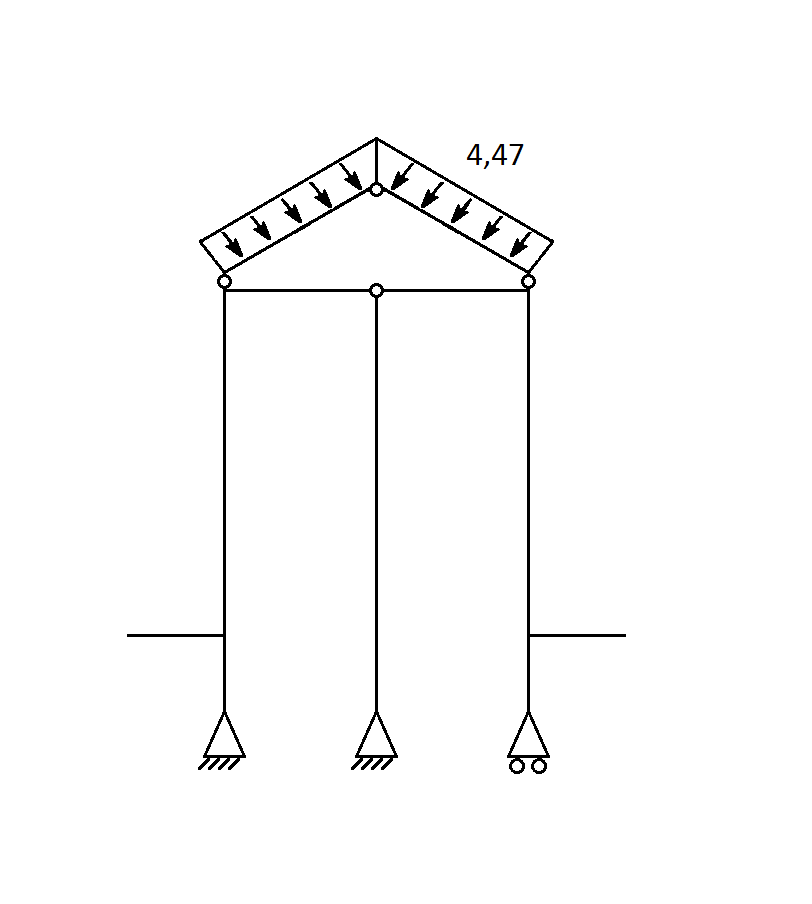
\includegraphics[width=0.3\textwidth]{billeder/snelast.png}
	\caption{Snelast på det statiske system angivet i [$\frac{\text{kN}}{\text{m}}$]}
	\label{fig:snelast}
\end{figure}

\subsubsection{Vindlast}
For vindlasten regnes der en nettovindlast, hvilken regnes som summen af den udvendige og den indvendige vindlast.
\newline \indent{     }  For Strøybergs Palæ regnes der en nettovindlast for taget og for facaderne på bygningen, hvilket gøres for tre vindretninger, nord, øst og vest, da sydsiden af tilbygningen kommer i forlængelse af den allerede eksisterende bygning, og derfor formodes denne vindlast ikke at have en særlig betydning for tilbygningen.
\newline
\newline
Til at bestemme vindlasten på tilbygningens udvendige sider anvendes følgende formel:	
\begin{equation} 
	w_e = q_p(z_e)c_{pe}
\end{equation}

\begin{itemize}
	\item[-] $q_p$: Peakhastighedstrykket
	\item[-] $z_e$: Referencehøjden for det udvendige vindtryk, som er 19 m for taget og 16 m for facaderne
	\item[-] $c_{pe}$: Formfaktoren for det udvendige vindtryk
\end{itemize}

Til at bestemme vindlasten på tilbygningens indvendige sider anvendes følgende formel:
\begin{equation} 
	w_i = q_p(z_i)c_{pi}
\end{equation}
\begin{itemize}
	\item[-] $q_p$: Peakhastighedstrykket
	\item[-] $z_i$: Referencehøjden for det indvendige vindtryk, som sættes lig det udvendige for hhv. tag og facader $z_e$ \citep[ kapitel 7.2.9]{EU91}
	\item[-] $c_{pi}$: F{\tiny }ormfaktoren for det indvendige vindtryk
\end{itemize}

I Bilag A ses et beregningseksempel på bestemmelse af peakhastighedstrykket, $q_p$, og i Tabel \ref{tab:peak} ses værdierne for peakhastighedstrykket for alle tre vindretninger ved højderne 16 m og 19 m.
\begin{table}[htb]
\begin{center}
	\begin{tabular}{ c c c } 
		\hline
		Vindretning/Højden & $q_p [\frac{\text{kN}}{\text{m}^2}]$ ved 16 m & $q_p [\frac{\text{kN}}{\text{m}^2}]$ ved 19 m \\	\hline
		Vest & 0,54 & 0,58 \\	
		Øst & 0,43 & 0,46 \\
		Nord & 0,43 & 0,46 \\
	\end{tabular}
		\caption{Værdier for $q_p$}
		\label{tab:peak}
\end{center}
\end{table}

Peakhastighedstrykket skal nu anvendes, for at bestemme vindlasten på taget fra de tre vindretninger.
\newline
\newline
\textbf{Vindtryk på tag}
\newline
Først bestemmes de karakteristiske vindlaster ved at opstille en række vindtilfælde for henholdsvis tryk og sug. Tryk regnes altid positivt, og sug regnes altid negativt.


Da tilbygningen til Strøybergs Palæ får et sadeltag, anbefales det at dele taget ind i zoner efter Eurocode 1991. Bygningen tegnes i fuld størrelse, hvor længden \textit{e} er 25 m, og derfor er den nuværende bygning også medregnet i målene. For vindretningen $\theta = 0^{\circ}$ (gælder for vindretning fra vest og fra øst) skal bygningen deles ind som vist på Figur \ref{fig:opdeling}.  

\begin{figure}[htbp]
	\centering
	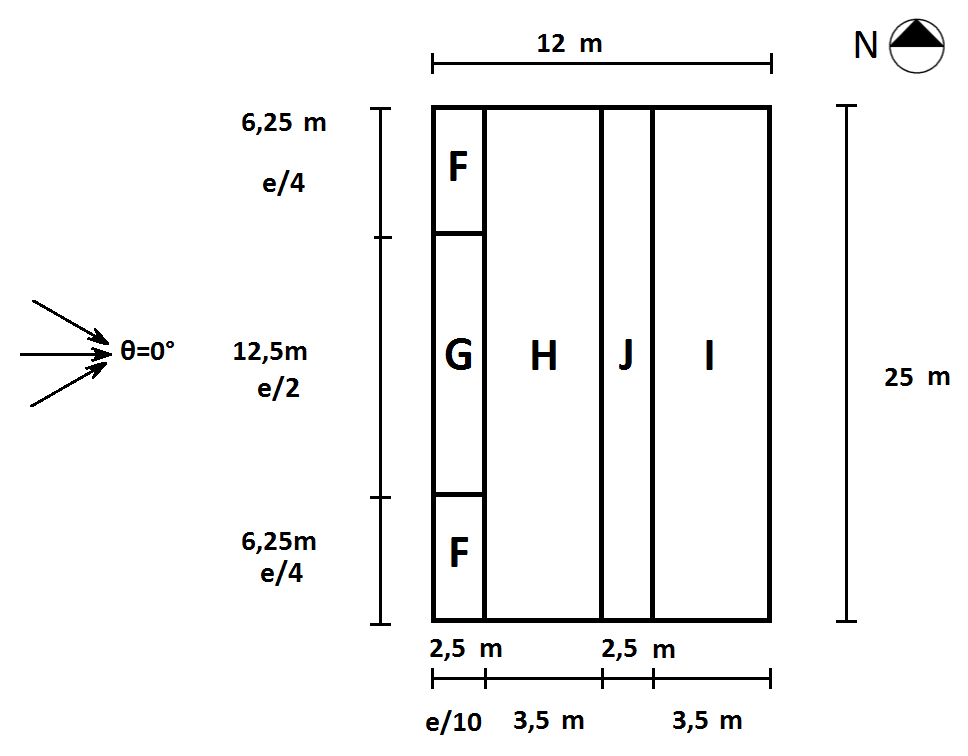
\includegraphics[width=0.6\textwidth]{billeder/opdeling.png}
	\caption{Opdeling af bygning, for vindretning fra øst og vest \citep[ kapitel 7.2.5]{EU91}}
	\label{fig:opdeling}
\end{figure}

Formfaktorerne, $c_{pe}$, for tagets zoner bestemmes ud fra Eurocode 1991. Her anvendes taghældningen på $\alpha = 26,\!57^{\circ}$, og der laves derfor lineær regression mellem $c_{pe}$ værdierne for vinklerne $15^{\circ}$ og $30^{\circ}$, efter anbefaling af Eurocode 1991 \citep[ tabel 7.4a kapitel 7.2.5]{EU91}. For $\theta = 0^{\circ}$ skifter trykket hurtigt mellem positive og negative værdier i vindsiden, ved en taghældning mellem $\alpha = -5^{\circ}$ til $+ 45^{\circ}$, og derfor skal der regnes for både positive og negative formfaktorværdier. 
\newline \indent{     }  Nedenfor er et beregningseksempel af formfaktoren.


\underline{Zone F for vind fra vest}
\newline
Ud fra Eurocode 1991 \citep[ tabel 7.4a kapitel 7.2.5]{EU91} findes de negative værdier for zone F ved $15^{\circ}$ og $30^{\circ}$. Her ud fra laves lineær regression, og $c_{pe,10,neg}$ bestemmes:
\begin{equation}
	c_{pe,10,neg} = -0,\!59
\end{equation}

Ligeledes gøres for de positive værdier for zone F ved $15^{\circ}$ og $30^{\circ}$, og $c_{pe,10,pos}$ bestemmes:
\begin{equation}
	c_{pe,10,pos}=0,\!59
\end{equation}

De beregnede værdier for formfaktorerne ses i Tabellerne \ref{tab:cc} og \ref{tab:kk}. 


De udvendige vindtryk beregnes ved formel 6.28. Værdierne findes alle i Bilag F punkt 2. 


De indvendige vindtryk skal nu bestemmes, da de virker på samme tid som de udvendige vindtryk.


Der findes to måder til bestemmelse af formfaktoren, $c_{pi}$, for indvendig vind. I dette projekt anvendes den forsimplede metode, hvor $c_{pi}$ regnes til at være den mindst gunstige af + 0,2 og - 0,3 \citep[Kapitel 7]{EU91}. Værdierne for formfaktoren ses i Tabellerne \ref{tab:cc} og \ref{tab:kk}.


Herefter kan de indvendige vindtryk beregnes ved formel 6.29.

\begin{table}[H]
	\begin{center}
		\begin{tabular}{ c c c c c } 
			\hline
			\multirow{2}{*}{Zone/Formfaktor} & \multicolumn{2}{l}{$c_{pe,10 udvendig}$} & \multicolumn{2}{l}{$c_{pe,10 indvendig}$} \\ 
			& Positiv & Negativ & Positiv & Negativ \\ \hline
			F & 0,59 & -0,59 & 0,20 & -0,30 \\
			G & 0,59 & -0,57 & 0,20 & -0,30 \\
			H & 0,35 & -0,22 & 0,20 & -0,30 \\ 
			I & 0,00 & -0,40 & 0,20 & -0,30 \\	
			J & 0,00 & -0,61 & 0,20 & -0,30 \\	
		\end{tabular}
		\caption{Værdier for $c_{pe,10}$ på udvendige og indvendige tagoverflader for vind fra vest og øst, vindretning $0^{\circ} = 180^{\circ}$ på taget}
		\label{tab:cc}
	\end{center}
\end{table}

\begin{table} [H]
	\begin{center}
		\begin{tabular}{ c c c c } 
			\hline
			\multirow{2}{*}{Zone/Formfaktor} & $c_{pe,10 udvendig}$ & \multicolumn{2}{l}{$c_{pe,10 indvendig}$} \\	
			& Negativ & Positiv & Negativ \\ \hline
			F & -1,15 & 0,20 & -0,30 \\	
			G & -1,38 & 0,20 & -0,30 \\ 
			H & -0,75 & 0,20 & -0,30 \\ 
			I & -0,50 & 0,20 & -0,30 \\	
		\end{tabular}
		\caption{Værdier for $c_{pe,10}$ på udvendige og indvendige tagoverflader for vind fra nord, vindretning $90^{\circ}$ på taget}
		\label{tab:kk}
	\end{center}
\end{table}

For at bestemme nettovindtrykket skal der opstilles en række tilfælde for, hvordan det udvendige vindtryk og det indvendige vindtryk kan optræde.  
\newline
\newline
Der opstilles fire vindkombinationer for hver vindretning:
\begin{enumerate}
	\item Tryk udvendigt på FGH + sug for JI og invendigt sug
	\item Tryk udvendigt på FGH + sug for JI og invendigt tryk
	\item Sug udvendigt for FGH + tryk på JI og invendigt sug
	\item Sug udvendigt for FGH + tryk på JI og invendigt tryk
\end{enumerate}

Nedenfor laves et beregningseksempel med vind fra vest med vindkombination 1 for zone F. De resterende værdier kan ses i Tabel \ref{tab:bb}.
\newline
\newline
Vindlasten skal omregnes til en linjelast, hvorfor der multipliceres med længden mellem bjælkerne, 6,25 m.
\begin{equation} 
	w_F = (w_{e,F}-w_{i,F}) \SI{6,25}{m}
\end{equation}

\begin{itemize}
	\item[-] $w_{e,F}$: Udvendigt vindtryk for zone F = $0,\!34 \frac{\text{kN}}{\text{m}^2}$
	\item[-] $w_{i,F}$: Indvendigt vindtryk for zone F = $-0,\!17 \frac{\text{kN}}{\text{m}^2}$
\end{itemize}

\begin{equation} 
	w_F = (0,\!34 \frac{\text{kN}}{\text{m}^2} - (-0,\!17 \frac{\text{kN}}{\text{m}^2})\cdot \SI{6,25}{m} = 3,\!20 \frac{\text{kN}}{\text{m}}
\end{equation}

For alle vindretningerne anvendes vindkombination 1 til videre beregning, og disse laster ses i Tabel \ref{tab:bb}. 

\begin{table}[htb]
	\begin{center}
		\begin{tabular}{ c c c c } 
			\hline
			Zone/Vindretning & Vest & Øst & Nord \\
			& w $[\frac{\text{kN}}{\text{m}}]$ & w $[\frac{\text{kN}}{\text{m}}]$ & w $[\frac{\text{kN}}{\text{m}}]$ \\ \hline
			F & 3,20 & 2,56 & -2,45 \\
			G & 3,20 & 2,56 & -3,80 \\	
			H & 2,37 & 1,89 & -1,31 \\ 	
			I & -0,36 & -0,29 & -0,58 \\
			J & -1,14 & -0,91 & - \\
		\end{tabular}
		\caption{Værdier for nettovindtryk på taget}
		\label{tab:bb}
	\end{center}
\end{table}

Fra Tabel \ref{tab:bb} ses, at værdierne for vest er større i forhold til værdierne for øst. Det formodes derfor, at vindlasten er mere kritisk ved vind fra vest, og der ses fremover bort fra vinden fra øst i projektet. I tabellen ses det ligeledes, at værdierne for nord alle er negative, hvilket skyldes at vinden fra nord kun kan påvirke taget med sug, og dermed ses der i denne rapport også bort fra denne. 
\newline \indent{     }  Derfor anvendes værdierne for vest til de videre beregninger, når der skal opstilles lastkombinationer.


\textbf{Vindtryk på facaderne}
\newline
Vinden vil også påvirke Strøybergs Palæ på facader og endegavle, og derfor skal vindlasten også beregnes for de lodrette vægge.
\newline \indent{     }  Nettovindtrykket på facaderne beregnes på samme måde som nettovindtrykket for taget, dog tages der udgangspunkt i Eurocode 1991 \citep[ tabel 7.1]{EU91}. Længden af bygningens facader skal anvendes, og igen bruges den fulde længde af bygningen, der består af den nuværende bygning samt tilbygningen, hvilket giver længden 25 m. 


For vindretning $\varphi = 0^{\circ}$ for vind fra vest og $\varphi = 180^{\circ}$ for vind fra øst gælder at $b$ = 25 m, $d$ = 12 m og højden $h$ = 16 m. Bygningen skal igen opdeles i nogle zoner, både for vind fra vest, øst og nord, hvor zonerne D og E ses på Figur \ref{fig:vindvest} og \ref{fig:vindost}, mens zonerne A, B og C kan ses i Eurocode 1991 \citep [kapitel 7.2.2 figur 7.5]{EU91}. Formfaktorværdierne findes i Tabel \ref{tab:ff} og \ref{tab:gg}.

\begin{figure}[htbp]\centering
	\begin{minipage}[b]{0.48\textwidth}\centering
		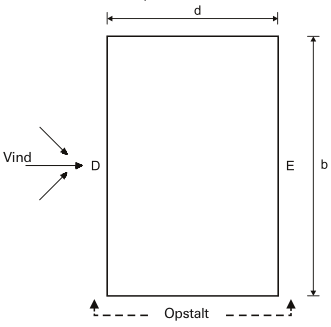
\includegraphics[width=0.9\textwidth]{billeder/vindvest1.png} %Venstre billede
	\end{minipage}\hfill
	\begin{minipage}[b]{0.48\textwidth}\centering
		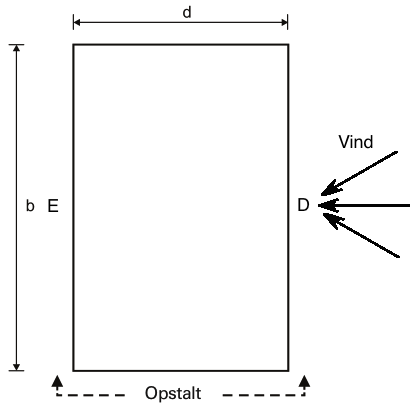
\includegraphics[width=0.9\textwidth]{billeder/vindost1.png} %Højre billede
	\end{minipage}\\ %Captions and labels
	\begin{minipage}[t]{0.48\textwidth}
		\caption{Vind på facaden fra vest \citep[ 7.2.2]{EU91}} %Venstre caption og label
		\label{fig:vindvest}
	\end{minipage}\hfill
	\begin{minipage}[t]{0.48\textwidth}
		\caption{Vind på facaden fra øst \citep[ 7.2.2]{EU91}} %Højre caption og label
		\label{fig:vindost}
	\end{minipage}
\end{figure}

Igen regnes der først en udvendige vindlast på facaderne og derefter en indvendig vindlast på facaderne, inden der opstilles en række vindkombinationer, hvor nettovindtrykket udregnes. For vindkombinationerne ses der bort fra siderne A, B og C, da den midterste ramme ligger 6,25 meter inde i konstruktionen og derfor ikke ligger i zonerne A, B eller C:
\begin{enumerate}
	\item Tryk udvendigt på D og sug indvendigt
	\item Sug udvendigt på E og sug indvendigt
	\item Tryk udvendigt på D og tryk indvendigt  
	\item Sug udvendigt på E og tryk indvendigt
\end{enumerate}

Der arbejdes videre med vindkombination 1, hvor den udvendige vind virker som tryk på siden D og sug på siden E og med en indre vindlast som sug.
\newline \indent{     }  Værdierne for nettovindtrykket kan ses i Tabel \ref{tab:hh}.

\begin{table}[htb]
	\begin{center}
		\begin{tabular}{ c c c c } 
			\hline
			\multirow{2}{*}{Zone/Formfaktor} & \multirow{2}{*}{$c_{pe,10}$ udvendig} & \multicolumn{2}{l}{$c_{pe,10}$ indvendig} \\ 
			& & Positiv & Negativ   		\\ \hline
			A & -1,20 & 0,20 & -0,30 \\	
			B & -0,80 & 0,20 & -0,30 \\	 
			D & 0,80 & 0,20 & -0,30 \\	
			E & -0,52 & 0,20 & -0,30 \\	
		\end{tabular}
		\caption{Værdier for $c_{pe,10}$ på facade for vind fra vest og øst, vindretning $0^{\circ} = 180^{\circ}$}
		\label{tab:ff}
	\end{center}
\end{table}

\begin{table}[htb]
	\begin{center}
		\begin{tabular}{ c c c c } 
			\hline
			\multirow{2}{*}{Zone/Formfaktor} & \multirow{2}{*}{$c_{pe,10}$ udvendig} & \multicolumn{2}{l}{$c_{pe,10}$ indvendig} \\ 
			& & Positiv & Negativ   		\\ \hline
			A & -1,20 & 0,20 & -0,30 \\	
			B & -0,80 & 0,20 & -0,30 \\	
			C & -0,50 & 0,20 & -0,30 \\	 
			D & 0,75 & 0,20 & -0,30 \\	
			E & -0,40 & 0,20 & -0,30 \\	
		\end{tabular}
		\caption{Værdier for $c_{pe,10}$ for vind fra nord, vindretning $90^{\circ}$}
		\label{tab:gg}
	\end{center}
\end{table}

\begin{table}[htb]
	\begin{center}
		\begin{tabular}{c c c c}
			\hline
			Zone/Vindretning & Vest & Øst & Nord \\ 
			& w $[\frac{\text{kN}}{\text{m}}]$ & w $[\frac{\text{kN}}{\text{m}}]$ & w $[\frac{\text{kN}}{\text{m}}]$ \\ \hline
			D & 3,69 & 2,95 & 2,14 \\ 
			E & -0,73 & -0,58 & -0,95 \\ 
		\end{tabular}
		\caption{Værdier for nettovindtryk på siderne}
		\label{tab:hh}
	\end{center}
\end{table}

Ud fra Tabel \ref{tab:hh} ses det, at værdierne for vest er størst. Det formodes igen, at vindlasten derfor er mere kritisk fra vest end for de to andre vindretninger, og der ses fremover bort fra vinden fra nord og øst. Derfor anvendes lasterne for vest videre, når der skal opstilles lastkombinationer for bygningen.
\newline \indent{     }  Disse linjelaster virker på højden af facaderne, der er siderne D og E, som hver er 16 m høje.


\textbf{Opsummering}
\newline
Det er nu bestemt i denne rapport, at der fokuseres på vind fra vest, hvor der optræder forskellige udvendige laster, mens den indre altid optræder som sug. Lasterne er omregnet til linjelaster ved at multiplicere med afstanden mellem rammerne, hvilken er 6,25 m. 
\newline
\newline
Systemet betragtes, hvor der laves beregninger for rammen i midten af konstruktionen, hvilken ligger 6,25 m inde på konstruktionen. Det betyder, rammen ligger mellem zone F og G (se Figur \ref{fig:opdeling}). Derfor udregnes et gennemsnit mellem værdierne for zonerne F og G ved vind på taget, da zonen E for siderne gælder for hele facaden. 
Dog ses det, at værdierne F og G for taget er ens, og dermed er gennemsnitsværdien lig med værdierne for F og G. 
\newline \indent{     }  De vindlaster der virker på det statiske system, som anvendes til videre beregninger, er illustreret på Figur \ref{fig:vindlast}. 

\begin{figure}[H]
	\centering
	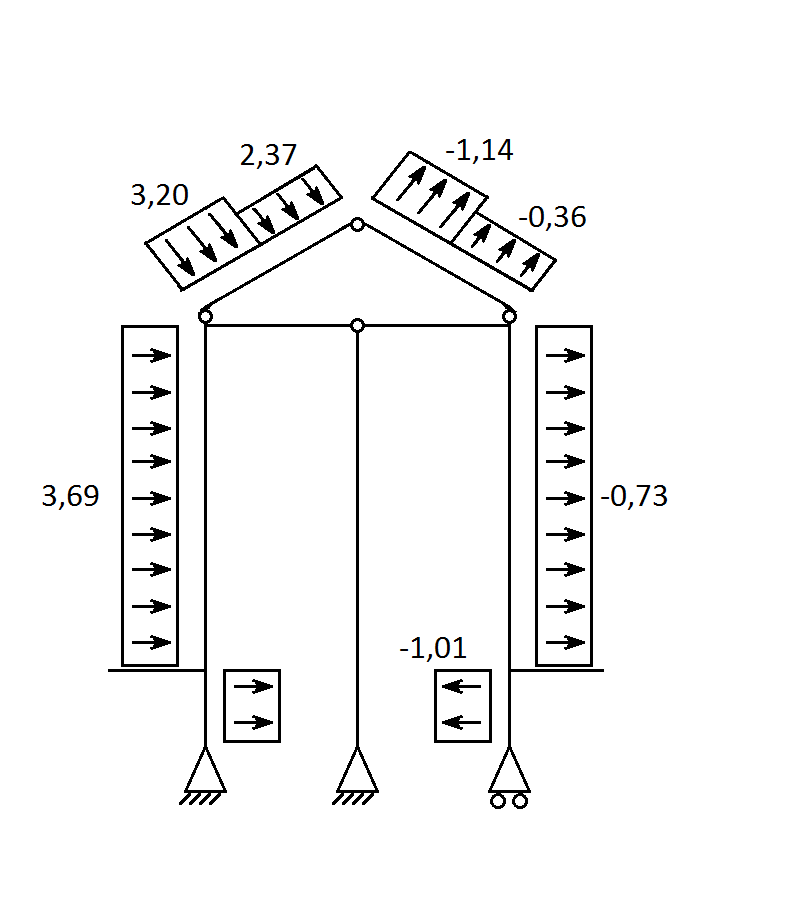
\includegraphics[width=0.4\textwidth]{billeder/vindlast.png}
	\caption{Vindlast på det statiske system angivet i [$\frac{\text{kN}}{\text{m}}$]}
	\label{fig:vindlast}
\end{figure}

\subsubsection{Nyttelast}
Ud fra Eurocode 1991 aflæses den jævnt fordelte last, $q_k$, for kategori A1, som er bolig og lokale adgangsveje, til $1,\!5 \frac{\text{kN}}{\text{m}^2}$ \citep[ tabel 6.2 kapitel 6.3.1.2]{EU91}. Lasten omregnes til en linjelast ved at multiplicere med afstanden mellem rammerne på 6,25 m. Hermed fås en linjelast på $9,\!37 \frac{\text{kN}}{\text{m}}$. 
\newline \indent{     }  Den nyttelast, der virker på det statiske system er illustreret på Figur \ref{fig:nyttelast}.

\begin{figure}[htbp]
	\centering
	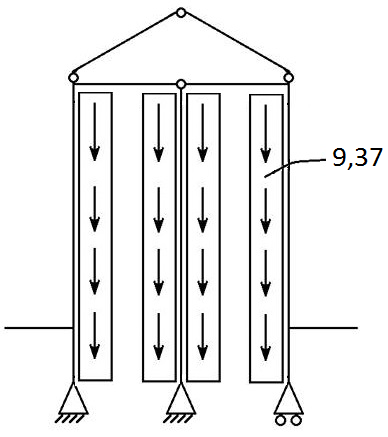
\includegraphics[width=0.3\textwidth]{billeder/nyttelast.png}
	\caption{Nyttelast på det statiske system angivet i [$\frac{\text{kN}}{\text{m}}$]}
	\label{fig:nyttelast}
\end{figure}

\section{Lastkombinationer}
Den karakteristiske egenlast, jordlast, vindlast, snelast og nyttelast er bestemt for tilbygningen til Strøybergs Palæ. Derfor opstilles en række lasttilfælde, for at finde de regningsmæssige laster, som skal anvendes til beregningerne af reaktioner. Lastkombinationerne opstilles ved at betragte tilbygningen i de områder, som er illustreret på Figur \ref{fig:omraader}.

\begin{figure}[H]
	\centering
	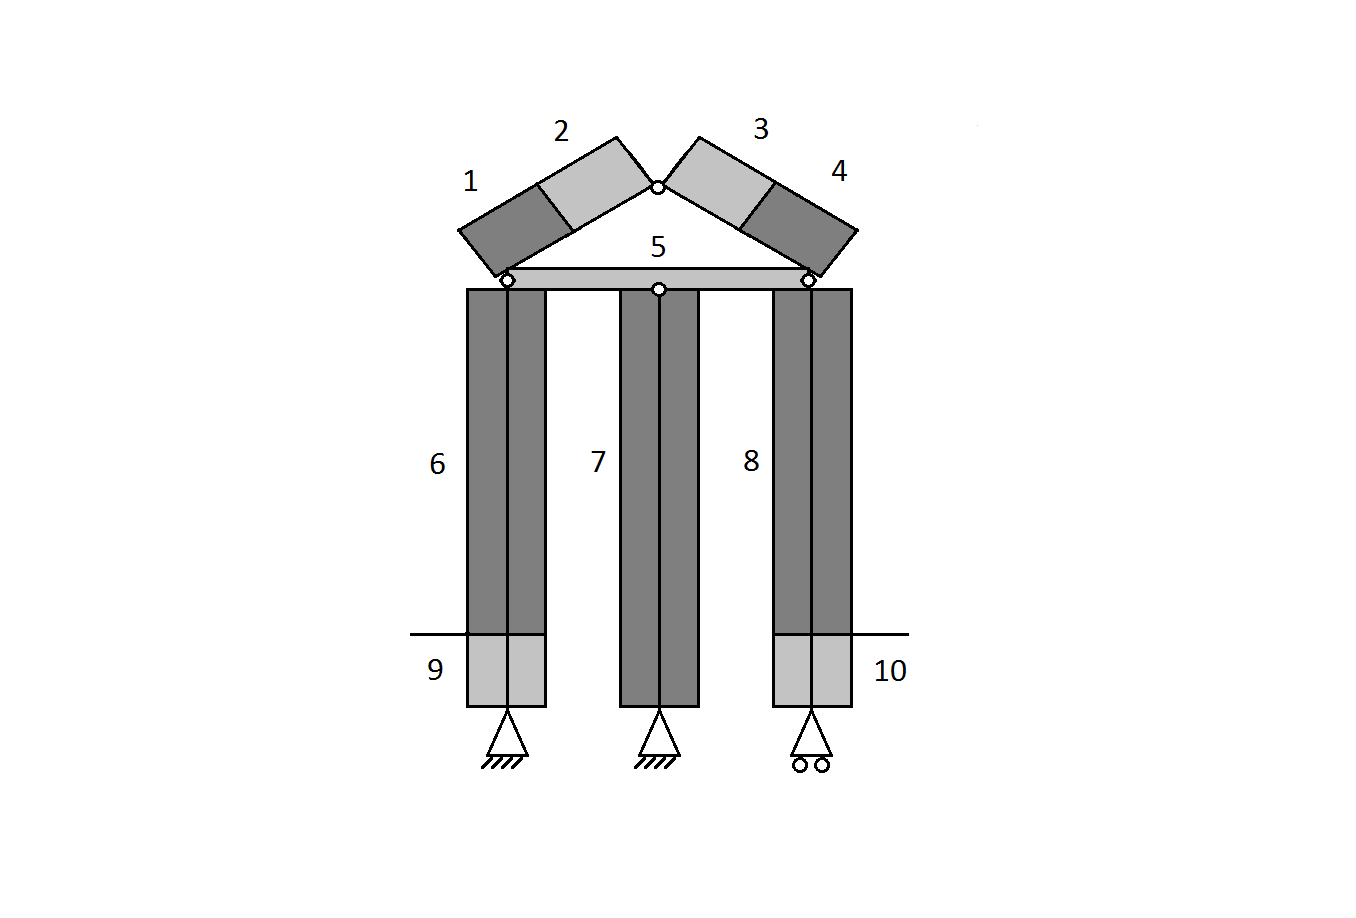
\includegraphics[width=0.3\textwidth]{billeder/indeling.png}
	\caption{Statisk system inddelt i områder}
	\label{fig:omraader}
\end{figure}

Ved et rigtigt byggeprojekt skal der opstilles lasttilfælde for alle tænkelige scenarier, som kan forekomme. For dette projekt er det dog ikke en mulighed, og derfor er der til videre beregninger valgt at fokusere på vindlast som den dominerende last. Hermed opstilles der følgende lastkombination for hvert område:
\begin{equation}
	E_d = \gamma_{G1} K_{FI} G_{K1}" + "\gamma_{G2} K_{FI} G_{K2}" + "\gamma_{Q1} K_{FI} Q_{K1}" + "\gamma_{Q2} \psi_{0,2} K_{FI} Q_{K2}" + "\gamma_{Q3} \psi_{0,3} K_{FI} Q_{K3}
\end{equation}

\begin{itemize}
	\item[-] $\gamma_G$: Partialkoefficient for permanente laster
	\item[-] $K_{FI}$: Konsekvensklasse
	\item[-] $G_K$: Karakteristisk værdi for permanent last
	\item[-] $\gamma_Q$: Partialkoefficient for variabel last
	\item[-] $Q_K$: Karakteristisk værdi for variabel last
	\item[-] $\psi$: Lastkombinationsfaktor 
\end{itemize}

Nedenfor gennemgås to beregningseksempler for den regningsmæssige last, med udgangspunkt i henholdsvis område 1 og 6. 

I område 1 optræder der vindlast, snelast og egenlast, og beregnes ved følgende:
\begin{equation}
	E_d = 1,\!0 \cdot 1,\!1 \cdot 4,\!89 \frac{\text{kN}}{\text{m}} "+" 1,\!5 \cdot 1,\!1 \cdot 3,\!20 \frac{\text{kN}}{\text{m}} "+" 1,\!5 \cdot 0 \cdot 1,\!1 \cdot 5,\!00 \frac{\text{kN}}{\text{m}}
\end{equation}

Herudfra kan lasten, der virker på løbende skrå længde, lasten der virker vinkelret på taget og lasten der virker på løbende vandret længde findes:
\begin{equation}
	\text{Egenlast} = 1,\!0 \cdot 1,\!1 \cdot 4,\!89 \frac{\text{kN}}{\text{m}} = 5,\!37 \frac{\text{kN}}{\text{m}}
\end{equation}
\begin{equation}
	\text{Vindlast} = 1,\!5 \cdot 1,\!1 \cdot 3,\!20 \frac{\text{kN}}{\text{m}} = 5,\!28 \frac{\text{kN}}{\text{m}}
\end{equation}
\begin{equation}
	\text{Snelast} = 1,\!5 \cdot 0 \cdot 1,\!1 \cdot 5,\!00 \frac{\text{kN}}{\text{m}} = 0,\!00 \frac{\text{kN}}{\text{m}}
\end{equation}

I område 6 optræder der vindlast, egenlast fra etagedæk, egenlast fra stålprofiler og nyttelast. Her er egenlasten for etagedæk og egenlasten fra stålprofilerne lagt sammen til 21,64 $\frac{\text{kN}}{\text{m}}$. Lastkombinationen opstilles som følgende:
\begin{equation}
	E_d = 1,\!0 \cdot 1,\!1 \cdot 21,\!64 \frac{\text{kN}}{\text{m}}" + "1,\!5 \cdot 1,\!1 \cdot 3,\!69 \frac{\text{kN}}{\text{m}}" + "1,\!5 \cdot 0,\!5 \cdot 1,\!1 \cdot 9,\!38 \frac{\text{kN}}{\text{m}}
\end{equation}

De laster der virker i vandret retning, altså i x-retningen, er vindlast:
\begin{equation}
	q_{x6} = 1,\!5 \cdot 1,\!1 \cdot 3,\!69 \frac{\text{kN}}{\text{m}} = 6,\!08 \frac{\text{kN}}{\text{m}}
\end{equation}

De laster der virker i lodret retning, er nyttelast, egenlast fra etagedæk samt egenlast fra stålprofiler:
\begin{equation}
	q_{y6} = 1,\!0 \cdot 1,\!1 \cdot 21,\!64 \frac{\text{kN}}{\text{m}} + 1,\!5 \cdot 0,\!5 \cdot 1,\!1 \cdot 9,\!38 \frac{\text{kN}}{\text{m}} = 31,\!54 \frac{\text{kN}}{\text{m}}
\end{equation}

Ovenstående beregninger gentages for hvert område på konstruktionen, og derfor regnes der for i alt 10 områder. De endelige laster der virker på konstruktionen, er angivet på Figur \ref{fig:laster}. 

\begin{figure}[htbp]
	\centering
	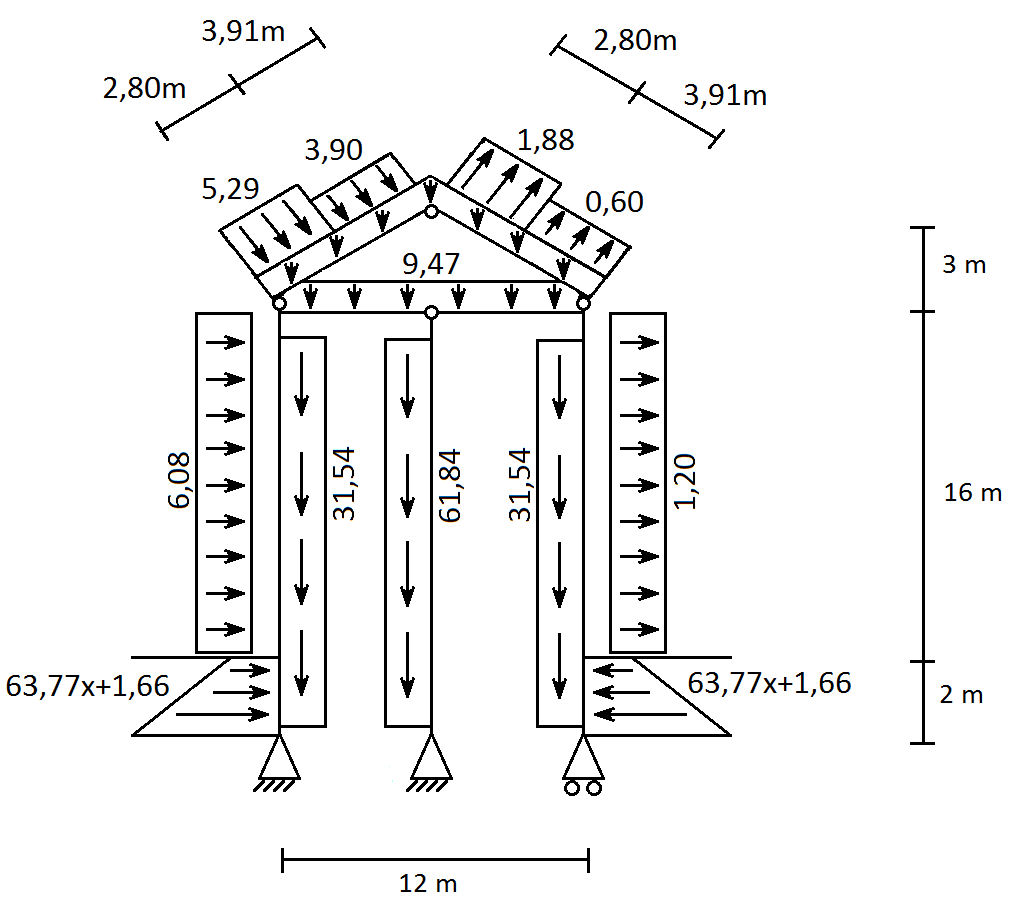
\includegraphics[width=0.7\textwidth]{billeder/vdom.png}
	\caption{Samlede laster på det statiske system med vind fra vest dominerende. Lasterne er angivet i [$\frac{kN}{m}$]}
	\label{fig:laster}
\end{figure}

Taget i bjælkekonstruktionen er forbundet til den resterende del af konstruktionen via charnierled. Lasterne, der virker på taget, vil dermed kunne overføres til den resterende del af konstruktionen som punktlaster med angrebspunkt i knudepunkterne, hvor charnierledene er. Reaktionerne og lasterne, som virker på taget, er illustreret på Figur \ref{fig:tagmedreaktioner}.

\begin{figure}[htbp]
	\centering
	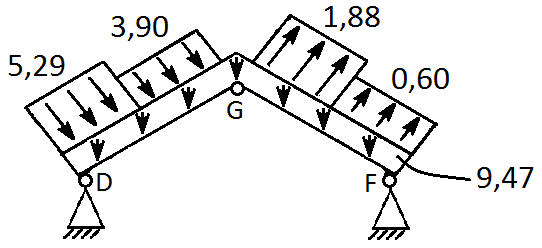
\includegraphics[width=0.4\textwidth]{billeder/tagmedreaktioner.png}
	\caption{Tag med laster og understøtninger. Lasterne er angivet i [$\frac{\text{kN}}{\text{m}}$]}
	\label{fig:tagmedreaktioner}
\end{figure}

De tre ligevægtsligninger anvendes til at bestemme punktlasterne. Dette gøres ved at udregne reaktionerne i punkterne D og F, hvor vindlasterne på taget omregnes til komposanter. Fritlegemediagrammet samt de laster på taget, der bruges til at udregne reaktionerne, er illustreret på Figur \ref{fig:fld}. 

\begin{figure}[htbp]
	\centering
	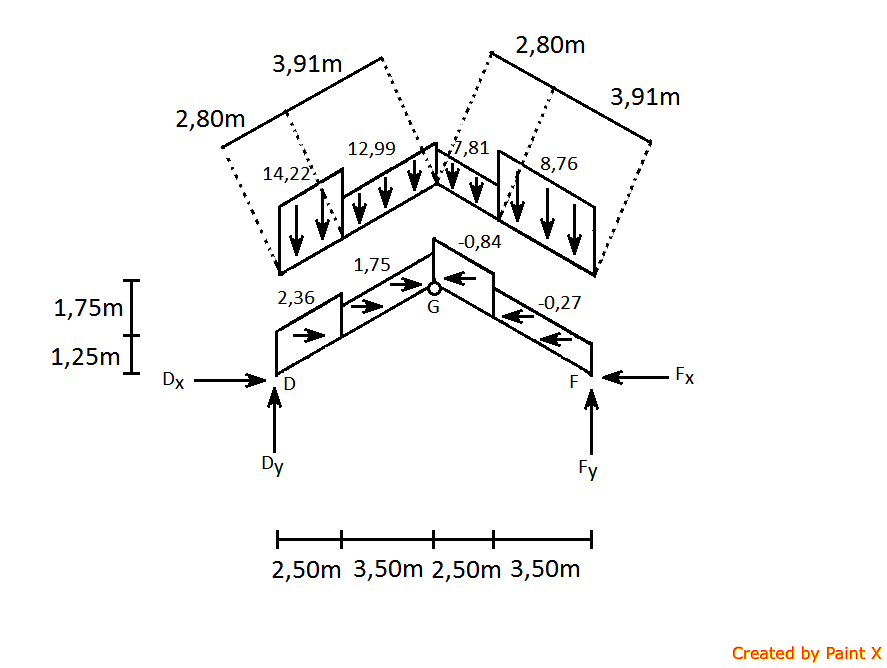
\includegraphics[width=0.8\textwidth]{billeder/fldtag.png}
	\caption{Fritlegemediagram af taget. Lasterne er angivet i [$\frac{\text{kN}}{\text{m}}$]}
	\label{fig:fld}
\end{figure}

Reaktionerne for taget kan dermed beregnes:
\begin{equation}
	\begin{split}
	\ALN{\text{D}}: 0 = &-h_{1y} \cdot \SI{2,80}{m} \cdot \frac{2,\!5 \text{m}}{2} - h_{2y} \cdot \SI{3,91}{m} \cdot (\SI{2,5}{m} + \frac{3,\!5 \text{m}}{2}) \\ & - h_{1x} \cdot \SI{2,80}{m} \cdot (\frac{1,\!25 \text{m}}{2}) - h_{2x} \cdot \SI{3,91}{m} \cdot (\SI{1,25}{m} + \frac{1,\!75 \text{m}}{2}) \\ & - h_{3y} \cdot \SI{2,80}{m} \cdot (\SI{6}{m} + \frac{2,\!5 \text{m}}{2}) - h_{4y} \cdot \SI{3,91}{m} \cdot (\SI{8,5}{m} + \frac{3,\!5 \text{m}}{2}) \\ & - h_{3x} \cdot \SI{2,80}{m} \cdot (\SI{1,25}{m} + \frac{1,\!75 \text{m}}{2}) - h_{4x} \cdot \SI{3,91}{m} \cdot (\frac{1,\!25 \text{m}}{2}) \\ & + \SI{12}{m} \cdot F_y
	\\ &
	F_y = \SI{39,74}{kN}
	\end{split}
\end{equation}

\begin{equation}
\begin{split}
	\rightarrow+: 0 = & -h_{1y} \frac{\text{kN}}{\text{m}} \cdot \SI{2,80}{m} - h_{2y} \frac{\text{kN}}{\text{m}} \cdot \SI{3,91}{m} - h_{3y} \frac{\text{kN}}{\text{m}} \cdot \SI{2,80}{m} -  h_{4y} \cdot \SI{3,91}{m} + D_y + F_y 
	\\ &
	D_y = \SI{52,45}{kN}
\end{split}
\end{equation}

\begin{equation}
\begin{split}
	\ALN{\text{G}}: 0 = & - h_{3y} \cdot \SI{2,80}{m} \cdot (\frac{2,\!5 \text{m}}{2}) - h_{4y} \cdot \SI{3,91}{m} \cdot (\SI{2,5}{m} + \frac{3,\!5 \text{m}}{2}) - h_{3x} \cdot \SI{2,80}{m} \cdot (\frac{1,\!25 \text{m}}{2}) \\& - h_{4x} \cdot \SI{3,91}{m} \cdot (\SI{1,25}{m} + \frac{1,\!75 \text{m}}{2}) + F_y \cdot \SI{6}{m} - F_x \cdot \SI{3}{m}
	\\ &
	F_x = \SI{49,57}{kN}
\end{split}
\end{equation}

\begin{equation}
\begin{split}
	\rightarrow+: 0 = & h_{1x} \cdot \SI{2,80}{m} + h_{2x} \cdot \SI{3,91}{m} - h_{3x} \cdot \SI{2,80}{m} - h_{4x} \cdot \SI{3,91}{m} - F_x + D_x
	\\ &
	D_x = \SI{32,74}{kN} 
\end{split}
\end{equation}

Disse reaktioner virker som punktlast på taget, og det endelige statiske system med de laster der skal bruges til at finde reaktioner for det statiske system, er illustreret på Figur \ref{fig:alle}. 

\begin{figure}[htbp]
	\centering
	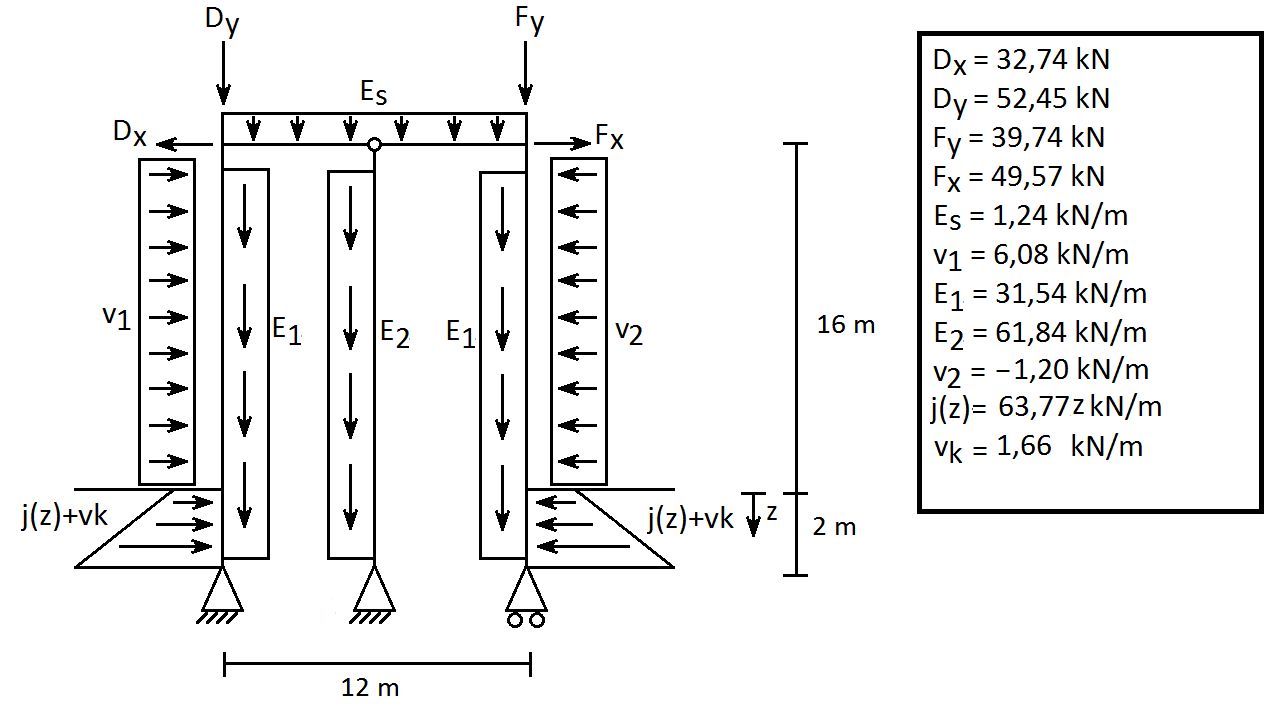
\includegraphics[width=0.8\textwidth]{billeder/endeligesystemmedlaster.png}
	\caption{Statisk system med punktlaster og linjelaster}
	\label{fig:alle}
\end{figure}